\section{Reformulating the Standard Model Lagrangian in VAM Units}\label{sec:lagrangian_vam}
The Standard Model Lagrangian encapsulates particle dynamics through symmetry-based field terms:
\begin{equation}
    \mathcal{L}_{\text{SM}} = -\frac{1}{4}F^{\mu\nu}F_{\mu\nu} + i\bar{\psi}\gamma^\mu D_\mu \psi + y_f \bar{\psi}\phi \psi + |D_\mu \phi|^2 - V(\phi)
\end{equation}
While mathematically elegant, these terms are not derived from first physical principles but are inserted axiomatically. The Vortex Æther Model (VAM) replaces this abstraction with a Lagrangian based on vortex dynamics, æther strain, and helicity conservation.

\subsection*{Core Assumptions}
\begin{itemize}
    \item The æther is a compressible, barotropic superfluid with stable vortex excitations.
    \item Particles are topologically stable vortex knots with quantized circulation.
    \item The Euler–Lagrange formalism applies to the action integral over fluid kinetic and potential energy densities.
    \item Helicity and vorticity are conserved modulo reconnection events.
\end{itemize}

\subsection*{Remarks on Spacetime Treatment}

In this model, the action integral is expressed as:
\[
    S = \int dt \int_{\mathbb{R}^3} \mathcal{L}(\vec{v}, \Phi, \rho_\text{\ae}, \dots) \, d^3x,
\]
reflecting a 3+1 decomposition with \textbf{absolute Newtonian time} and \textbf{Euclidean spatial geometry}.

Unlike relativistic field theories defined on Minkowski space \( \mathbb{R}^{1,3} \), the VAM adopts a \textbf{non-relativistic ontology}, where time is globally ordered and external to field dynamics.

This approach is consistent with established non-relativistic field theories, such as the Gross–Pitaevskii and hydrodynamic models for Bose–Einstein condensates, where space and time are decoupled and the Lagrangian formalism operates over \( \mathbb{R}^3 \times \mathbb{R} \)~\cite{Pethick2008BEC}.

Relativistic invariance in this context is regarded as an \textbf{emergent symmetry} that may arise at large scales or in specific limits of vortex behavior.

\subsection*{VAM-Reformulated Lagrangian}
Each term in the SM Lagrangian maps to a mechanical analog:

\begin{align*}
    \mathcal{L}_\text{VAM} &= \underbrace{-\frac{1}{4} \sum_{a} W^{a}_{\mu\nu} W^{a\mu\nu}}_{\text{Gauge field vorticity}}
    + \underbrace{\sum_{f} i \, m_f C_e r_c \, \bar{\psi}_f \gamma^\mu D_\mu \psi_f}_{\text{Fermion swirl propagation}} \\
    &- \underbrace{|D_\mu \phi|^2}_{\text{Æther strain field}}
    - \underbrace{V(\phi)}_{\text{Æther compression potential}}
    - \underbrace{\sum_f y_f \bar{\psi}_f \phi \psi_f + \text{h.c.}}_{\text{Mass coupling}}
    + \underbrace{\mathcal{H}_\text{topo}}_{\text{Vortex helicity term}}
\end{align*}

Where:
\[
    V(\phi) = -\frac{F^{\text{\ae}}_{\text{max}}}{r_c}|\phi|^2 + \lambda |\phi|^4
    \quad \text{and} \quad \mathcal{H}_\text{topo} = \int \vec{v} \cdot \vec{\omega} \, dV
\]
The full variational derivation of this Lagrangian—including Euler–Lagrange equations for velocity, scalar, and density fields—is provided in Appendix~\ref{sec:EL-derivation}.

\subsection{Gauge Fields as Vorticity Structures}
From Helmholtz’s theorem, the energy density in a vortex field is:
\begin{equation}
    \mathcal{L}_{\text{swirl}} = \frac{1}{2} \rho_\text{\ae} \left( |\vec{v}|^2 + \lambda |\nabla \times \vec{v}|^2 \right)
\end{equation}
Here, $\vec{v}$ is swirl velocity; $\lambda$ captures æther compressibility. Incompressible flows correspond to pure gauge configurations ($\nabla \cdot \vec{v} = 0$), while compressible strains allow field strength analogs.

\begin{figure}[H]
    \centering
    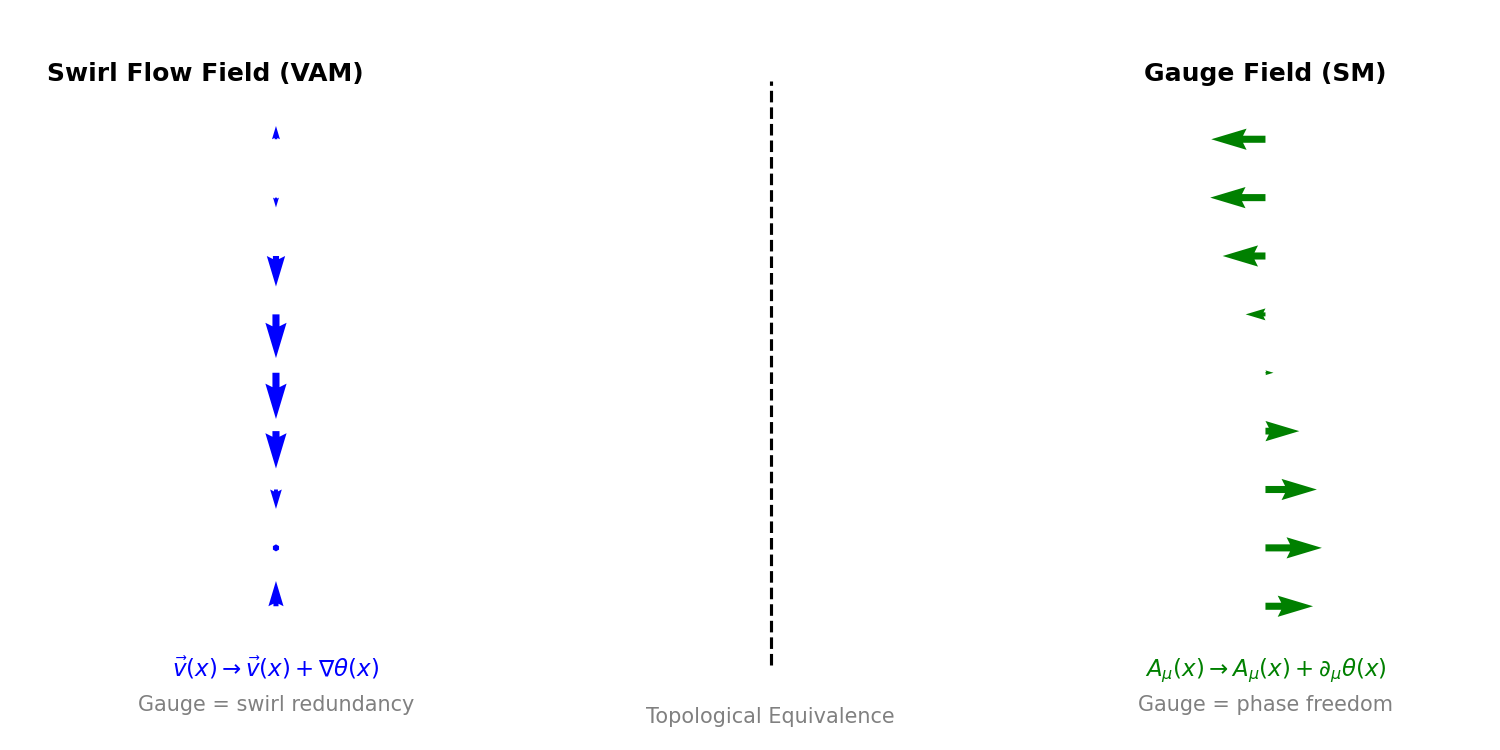
\includegraphics[width=0.95\textwidth]{images/gauge_swirl_equivalence}
    \caption{Analogy between gauge symmetry in the Standard Model and swirl invariance in the Vortex Æther Model (VAM). Both allow local reparameterizations that leave physical observables unchanged. Gauge symmetry in quantum field theory is structurally equivalent to potential-flow invariance in vortex dynamics.}
    \label{fig:gauge_swirl_equivalence}
\end{figure}

\begin{figure}[H]
    \centering
    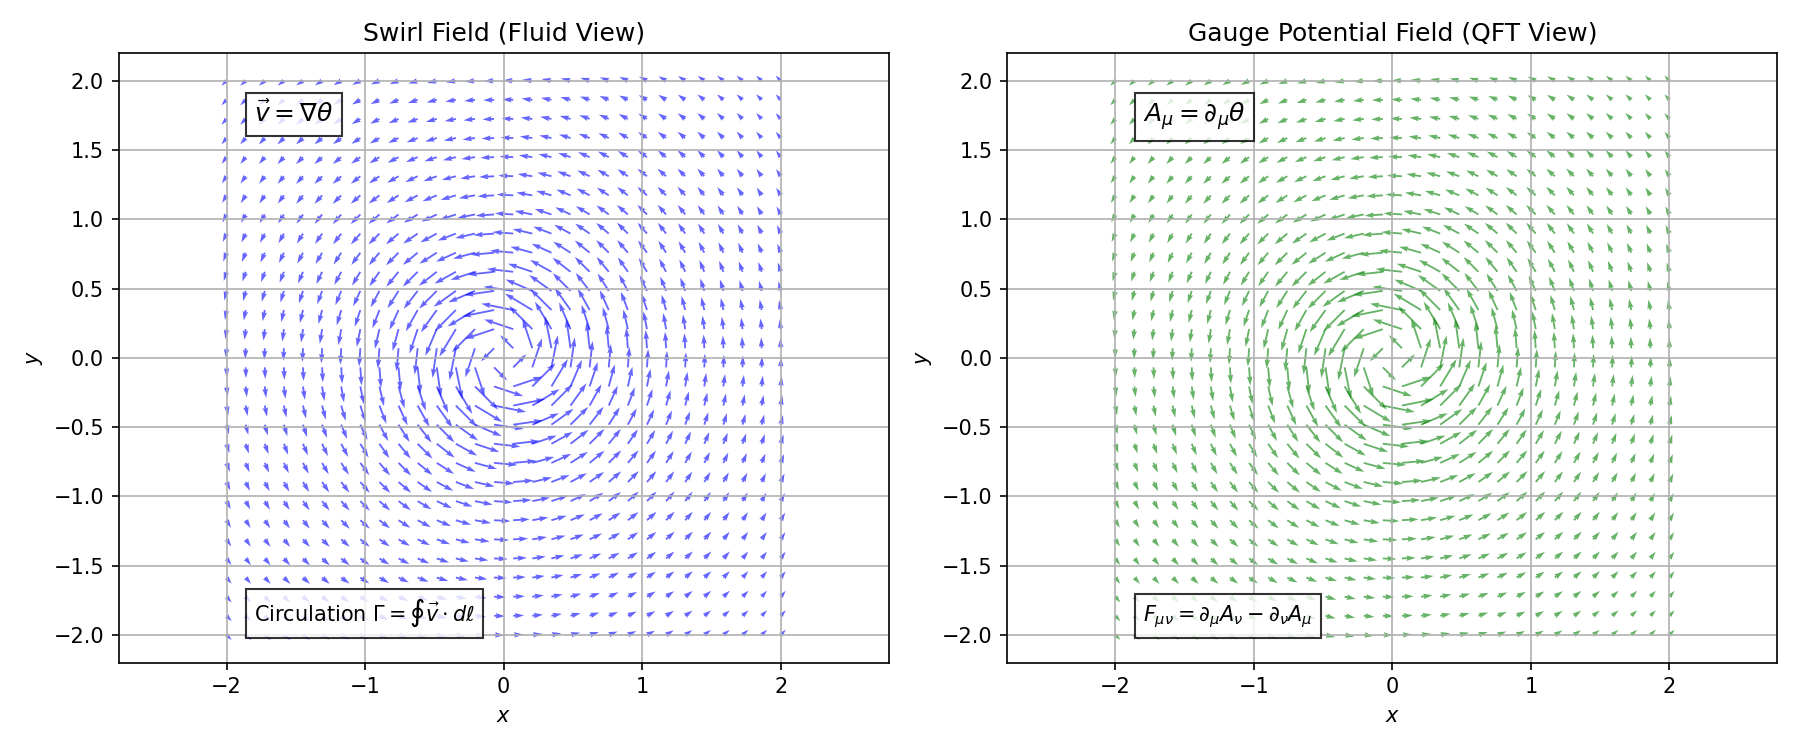
\includegraphics[width=0.9\linewidth]{images/SwirlVSGauge}
    \caption{
        Visual analogy between a fluid swirl field (left) and a gauge potential field in quantum field theory (right).
        Both fields depict circulation around a central core, but the left arises from mechanical vorticity in a compressible æther,
        while the right encodes electromagnetic or gauge interaction via abstract potential terms.
        This duality illustrates how local gauge invariance in QFT corresponds to conserved swirl topology in VAM.
    }
    \label{fig:swirl_gauge_analogy}
\end{figure}

\subsection{Fermion Kinetics via Swirl Propagation}
In the hydrodynamic formalism:
\begin{equation}
    \mathcal{L}_{\text{fermion}} = \rho_\text{\ae} C_e \Gamma \left( \psi^* \partial_t \psi - \vec{v} \cdot \nabla \psi \right)
\end{equation}
The convective derivative replaces $D_\mu$, and $\Gamma = 2\pi r_c C_e$ links to the particle’s spin-½ topology. Swirl modulates propagation analogous to minimal coupling.

\subsection{Mass from Helicity and Inertia}
The VAM mass term derives from vortex inertia under æther drag:
\begin{equation}
    m_f = \frac{\rho_{\ae} \Gamma^2}{3\pi r_c C_e^2} \quad\Rightarrow\quad \mathcal{L}_{\text{mass}} = -m_f \psi^* \psi
\end{equation}
This replaces abstract Yukawa interactions with fluidic resistance to internal swirl flow.

\subsection{Higgs Field as Æther Compression}
The standard Higgs potential $V(\phi) = -\mu^2|\phi|^2 + \lambda|\phi|^4$ becomes:
\begin{equation}
    V(\rho_\text{\ae}) = \frac{1}{2}K(\rho_\text{\ae} - \rho_0)^2 \quad\text{or}\quad V(\phi) = -\frac{F^{\text{\ae}}_{\text{max}}}{r_c} |\phi|^2 + \lambda |\phi|^4
\end{equation}
$K$ is the æther’s bulk modulus. The vacuum expectation value corresponds to equilibrium density, leading to spontaneous tension minima that stabilize particle structure.

\subsection{Topological Helicity and Knot Dynamics}
\begin{equation}
    \mathcal{H}_\text{topo} = \int \vec{v} \cdot \vec{\omega} \, dV
\end{equation}
This term tracks conservation of topological linkage and orientation. It becomes significant in processes involving particle transmutation, confinement, or decay.

\section{Helicity as a Chern--Simons Analog}

The helicity density term in the Vortex Æther Model (VAM),
\begin{equation}
\mathcal{L}_{\text{helicity}} = \lambda\, \vec{v} \cdot \vec{\omega},
\end{equation}
serves a central role in encoding the topological complexity of vortex configurations. Here, $\vec{\omega} = \nabla \times \vec{v}$ is the local vorticity field, and $\lambda$ is a coupling constant dependent on the æther's inertial density. However, this term is not merely phenomenological—it possesses a deep connection with topological field theory, specifically the Chern--Simons action.

In 3D gauge theories, the Abelian Chern--Simons action is given by:
\begin{equation}
S_{\text{CS}} = \int d^3x\, \epsilon^{ijk} A_i \partial_j A_k = \int \vec{A} \cdot (\nabla \times \vec{A})\, d^3x,
\end{equation}
which is formally analogous to the helicity integral in fluid dynamics:
\begin{equation}
\mathcal{H} = \int \vec{v} \cdot \vec{\omega}\, d^3x.
\end{equation}

In this analogy, the velocity field $\vec{v}$ plays the role of a gauge potential, and vorticity $\vec{\omega}$ becomes the field strength. This correspondence suggests that helicity is a conserved, quantized topological invariant under the transformation:
\begin{equation}
\theta(\vec{x}) \rightarrow \theta(\vec{x}) + \alpha(\vec{x}) \quad \Rightarrow \quad \vec{v} \rightarrow \vec{v} + \nabla \alpha,
\end{equation}
mirroring a $U(1)$ gauge transformation in QED.

Because the Chern--Simons term is not gauge invariant under large gauge transformations, its quantization ensures that the helicity integral remains invariant up to $2\pi n$ in units of a coupling constant. This provides a natural framework for explaining the quantized linking number $L_k$ of vortex knots in the VAM as a topological charge.

Thus, $\vec{v} \cdot \vec{\omega}$ is not merely a dynamical term, but encodes the fluid analog of a gauge-theoretic topological invariant \cite{moffatt1969degree, jackiw1990chern, verlinde2021qft}.


\subsection{Emergent Constants from Fluid Analogs}
Derivations of $\hbar_{\text{VAM}}$ and charge coupling follow:

\begin{align}
    \hbar_{\text{VAM}} &= m_f C_e r_c \\
    e^2 &= 8\pi m_e C_e^2 r_c \\
    \Gamma &= \frac{h}{m} = 2\pi r_c C_e
\end{align}

These reinterpret Planck-scale constants as emergent quantities from measurable æther dynamics and flow quantization, aligning with results from BEC vortex systems \cite{Pethick2008BEC, Donnelly1991QuantizedVortices}.

In this formulation, each field and interaction of the Standard Model gains a mechanical analog in the æther medium. The Lagrangian no longer relies on abstract symmetry principles alone, but instead emerges from vortex dynamics, circulation, density modulation, and topological structure within a unified fluid framework.


\subsection*{Mathematical Derivation of the VAM-Lagrangian}

Kinetic energy of a vortex structure, or the local energy density in a vortex field:

\[
    \mathcal{L}_\text{kin} = \frac{1}{2}\rho_\text{\ae} C_e^2
\]

Field energy and gauge terms, field tensors follow from Helmholtz vorticity:

\[
    \mathcal{L}_\text{veld} = -\frac{1}{4}F_{\mu\nu}F^{\mu\nu}
\]

Mass as inertia from circulation, where the fermion mass is determined by circulation:
\[
    \Gamma = 2\pi r_c C_e \quad\Rightarrow\quad m \sim \rho_\text{\ae} r_c^3
\]

Pressure and stress potential of æther condensate, where the pressure balance is described by the stress field:
\[
    V(\phi) = -\frac{F^{\text{\ae}}_{\text{max}}}{r_c}|\phi|^2 + \lambda|\phi|^4
\]

Topological terms for the conservation of vortex fields helicity:
\[
    \mathcal{H} = \int \vec{v}\cdot\vec{\omega}\, dV
\]

\begin{table}[H]
    \centering
    \footnotesize
    \renewcommand{\arraystretch}{1.4}
    \begin{tabular}{|l|l|l|l|}
        \hline
        \textbf{SM Term} & \textbf{Mathematical Form} & \textbf{VAM Analog} & \textbf{Fluid-Dynamic Interpretation} \\
        \hline
        \makecell[l]{Fermion Kinetic \\ Term} &
        $\bar{\psi}(i\gamma^\mu D_\mu)\psi$ &
        $\rho_\text{\ae} \vec{v}^2$ &
        \makecell[l]{Kinetic energy of topological vortex knot (fermion)} \\
        \hline
        \makecell[l]{Gauge Field \\ Kinetic Term} &
        $-\frac{1}{4}F_{\mu\nu}F^{\mu\nu}$ &
        $\rho_\text{\ae} (\vec{v} \cdot \nabla \times \vec{v})$ &
        \makecell[l]{Swirl helicity (fluid analog of gauge field energy)} \\
        \hline
        Fermion Mass Term &
        $m\bar{\psi}\psi$ &
        $\rho_{core} C_e^2$ &
        \makecell[l]{Core pressure from tangential circulation of vortex} \\
        \hline
        \makecell[l]{Higgs Field \\ Kinetic Term} &
        $\frac{1}{2}(\partial_\mu \phi)^2$ &
        $\frac{1}{2}(\nabla \phi)^2$ &
        \makecell[l]{Elastic strain in scalar potential field of Æther} \\
        \hline
        Higgs Potential &
        $V(\phi) = -\mu^2\phi^2 + \lambda \phi^4$ &
        $\lambda \phi^4 (1 - \phi^2/F^{\text{\ae}}_{\text{max}}^2)$ &
        \makecell[l]{Compressibility-induced pressure potential} \\
        \hline
        Yukawa Coupling &
        $y\bar{\psi}\phi\psi$ &
        $\rho_\text{\ae} \phi$ &
        \makecell[l]{Topological mass coupling via scalar compression} \\
        \hline
        Gauge Coupling &
        $D_\mu = \partial_\mu - igA_\mu$ &
        $\vec{v} + \vec{A}_{\text{swirl}}$ &
        \makecell[l]{Swirl-mediated interaction velocity} \\
        \hline
        QCD Term &
        $G_{\mu\nu}^a G^{\mu\nu}_a$ &
        -- &
        \makecell[l]{Conservation of angular momentum in \\ trichiral vortex flows} \\
        \hline
        EM Coupling &
        $q\bar{\psi}\gamma^\mu A_\mu \psi$ &
        $\Gamma \cdot \chi$ &
        \makecell[l]{Charge as circulation magnitude and chirality} \\
        \hline
        Chiral Asymmetry &
        -- &
        Knot handedness &
        \makecell[l]{Topological chirality determines weak \\ interaction selectivity} \\
        \hline
    \end{tabular}
    \caption{Comparison of Standard Model Lagrangian terms with their VAM fluid-dynamic analogs.}
    \label{tab:SMtoVAM}
\end{table}


\subsection*{Supporting Experimental and Theoretical Observations}
The VAM is consistent with experimentally and theoretically confirmed phenomena such as vortex stretching, helicity conservation and mass-inertia couplings \cite{batchelor1953,vinen2002,bewley2008,moffatt1969,kleckner2013,scheeler2014,bartlett1986}.

This reformulation offers a physically intelligible and topologically rich counterpart to the Standard Model—one grounded in measurable fluid properties, rather than abstract gauge symmetries alone.

\section{Quantized Swirl Fields via Mode Expansion}

In conventional quantum field theory (QFT), the quantization of fields arises from harmonic mode expansions that map classical field solutions to quantum operators. Each normal mode of the field is associated with a pair of creation and annihilation operators, leading to a discrete energy spectrum. Inspired by this formalism, we propose an analogous quantization framework for the Vortex Æther Model (VAM), in which the fluid velocity field $\vec{v}(\vec{x}, t)$ is expanded in a basis of knotted vortex modes.

We define the swirl field operator as:
\begin{equation}
\vec{v}(\vec{x}, t) = \sum_n \left[ \vec{v}_n(\vec{x})\, a_n e^{-i\omega_n t} + \vec{v}_n^*(\vec{x})\, a_n^\dagger e^{i\omega_n t} \right],
\end{equation}
where $a_n$ and $a_n^\dagger$ denote the annihilation and creation operators for the $n$-th vortex mode, and $\omega_n$ is the angular frequency associated with the core circulation and knot topology.

Each $\vec{v}_n(\vec{x})$ represents a quantized topological excitation of the æther, corresponding to distinct vortex knot configurations or harmonics. These excitations can be labeled by their helicity, circulation quantum $\Gamma_n$, and winding number $L_k$, akin to quantized angular momentum states in quantum mechanics.

This expansion justifies the discrete energy spectrum observed in vortex-based particle models. For example, the energy of a vortex excitation can be defined analogously to a harmonic oscillator:
\begin{equation}
E_n = \hbar_{\text{VAM}} \omega_n = \rho_{\ae} \Gamma_n r_c^2 \omega_n,
\end{equation}
with $\hbar_{\text{VAM}}$ interpreted as a fluid-circulation-based quantum of action:
\begin{equation}
\hbar_{\text{VAM}} \equiv \rho_{\ae} \Gamma_n r_c^2.
\end{equation}

This formulation is aligned with canonical quantization procedures in QFT \cite{verlinde2021qft}, and also with the formal mode expansions of collective excitations in superfluid systems \cite{pethick2002bose} and knotted vortex models \cite{kleckner2013creation}. It enables a rigorous interpretation of particles as quantized, topologically distinct excitations of the swirl field.

This framework can also extend to include internal excitation spectra of vortex cores, thereby suggesting a natural pathway for encoding flavor states and even mixing matrices in terms of mode-coupled vortex families.

